\chapter{Transient flow and heat equations - the Rayleigh-Benard instability}

\modinfo{Directory}{RayleighBenard}
\modinfo{Solvers}{\Idx{HeatSolve}, \Idx{FlowSolve}}
\modinfo{Tools}{\Idx{ElmerGrid},Editor}
\modinfo{Dimensions}{2D, Transient}

\subsection*{Case definition}
\begin{flushleft}
This tutorial is about simulating the developing of the Rayleigh-Benard instability in a rectangular domain 
(Figure \ref{fg:rb_geometry}) of dimensions 0.01 m height and 0.06 m length. The simulation is performed with water and the needed material parameters of water are presented in Table \ref{tb:matpar}. The temperature difference between the upper and lower boundary is set to 0.5 so that lower one has the temperature of  283.5 K and the upper one has the temperature of 283 K.



The density of water is inversely proportional to its temperature. Thus, heated water starts to flow upwards, and colder downwards due to gravity. 
In this case we assume that the \Idx{Boussinesq} approximation is valid for thermal incompressible fluid flow. In other words, the density of the term $\rho$$\vec{f}$ in the incompressible Navier-Stokes equation can be redefined by the Boussinesq approximation
\begin{displaymath}
\rho = {\rho}_0(1-\beta(T-{T}_0))
\end{displaymath}
where $\beta$ is the heat expansion coefficient and the subscript 0 refers to a reference state.


\begin{figure}[h]
\centering
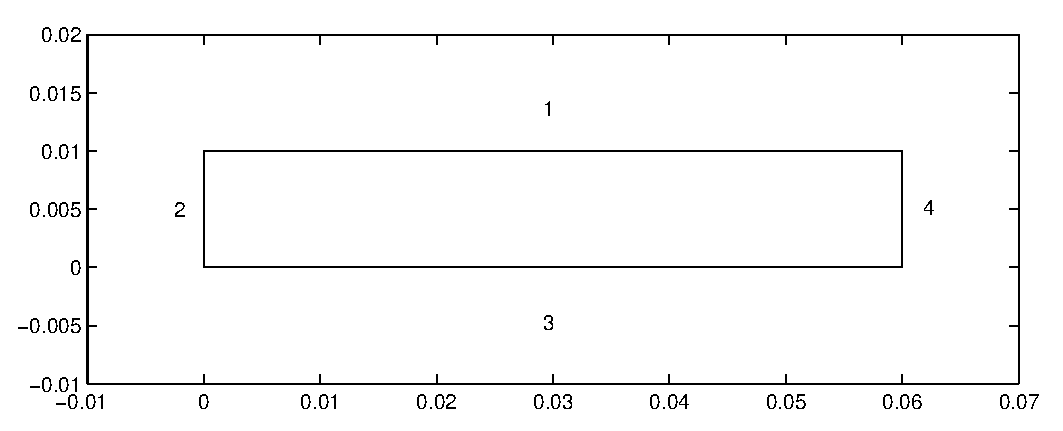
\includegraphics[width=150 mm, height=55 mm]{rb_geometry}
\caption{Domain.}\label{fg:rb_geometry}
\end{figure}  


\begin{table}[h]
\caption{Material parameters.}
\label{tb:matpar}
\begin{center}
\begin{tabular}{ll} \hline
parameter  & value \\ \hline
density & 1000 kg/m$^{3}$ \\
viscosity & 1040e-6 Ns/m$^{2}$ \\
heat capacity & 4190 J/(kg$\cdot$K) \\
heat conductivity & 0.6 W/(m$\cdot$K)       \\
heat expansion coefficient & 1.8e-4 K$^{-1}$      \\ 
reference temperature & 283 K       \\ \hline
\end{tabular}
\end{center}
\end{table}

\subsection*{Solution procedure}

The mesh has been constructed in advance and it consists of 2646 elements. 
The mesh files locate under the directory {\tt Mesh}.
\ttbegin
Header
  Mesh DB "." "Mesh"
  Include Path ""
  Results Directory ""
End
\ttend

The simulation is carried out in 2-dimensional cartesian coordinates. Newmark time-stepping method is selected with 200 steps and with step size of two seconds. In addition, we have to set the value {\tt Transient} for the keyword {\tt Simulation Type}.

\ttbegin
Simulation
  Coordinate System = "Cartesian 2D" 
  Coordinate Mapping(3) = 1 2 3
  Timestepping Method = "Newmark"
  Newmark Beta = 1
  Timestep Intervals(1) = 200
  Timestep Sizes(1) = 2
  Output Intervals(1) = 1
  Simulation Type = "Transient" 
  Steady State Max Iterations = 10
  Solver Input File = "RayleighBenard.sif"
  Output File = "RayleighBenard.result" 
  Post File = "RayleighBenard.ep" 
End
\ttend

Only one body is needed during the simulation.

\ttbegin
Body 1
  Equation = 1
  Material = 1
  Body force = 1
  Initial Condition = 1
End
\ttend

We assume that the Boussinesq approximation is valid.

\ttbegin
Body Force 1
  Boussinesq = True
End
\ttend

In next section the needed initial conditions are defined.

\ttbegin
Initial Condition 1
  Temperature = 283
  Velocity 1 = 1.0e-9
  Velocity 2 = 0
End
\ttend

The equations of the model are coupled and that is why the convection is computed.

\ttbegin
Equation 1
  Navier-Stokes = True
  Heat Equation = True
  Convection = "Computed"
End
\ttend

We must also define the material parameters of water.

\ttbegin
Material 1
  Density = 1000
  Viscosity = 1040e-6
  Heat Capacity = 4190
  Heat Conductivity = 0.6
  Heat Expansion Coefficient = 1.8e-4
  Reference Temperature = 283
End
\ttend

The heat equation is solved first using direct solver. 

\ttbegin
Solver 1
  Equation = "Heat Equation"
  Stabilize = Logical True
  Nonlinear System Max Iterations = 1
  Nonlinear System Convergence Tolerance = 1.0e-6
  Nonlinear System Newton After Iterations = 3 
  Nonlinear System Newton After Tolerance = 1.0e-3
  Nonlinear System Relaxation Factor = 1
  Linear System Solver = "Direct"
  Linear System Iterative Method = "BiCGStab"
  Linear System Convergence Tolerance = 1.0e-12
  Linear System Max Iterations = 100
  Steady State Convergence Tolerance = 1.0e-6
End
\ttend

The second solver solves the incompressible Navier-Stokes equation. We have used iterative solver this time. Also all the convergence criterions are defined in the following section.  

\ttbegin
Solver 2
 Equation = "Navier-Stokes"
 Stabilize = Logical True
 Nonlinear System Max Iterations = 1
 Nonlinear System Convergence Tolerance = 1.0e-6
 Nonlinear System Newton After Iterations = 3
 Nonlinear System Newton After Tolerance = 1.0e-3
 Nonlinear System Relaxation Factor = 1
 Linear System Solver = "Iterative"
 Linear System Iterative Method = "BiCGStab"
 Linear System Convergence Tolerance = 1.0e-9
 Linear System Max Iterations = 100
 Linear System Preconditioning = ILU1
 Steady State Convergence Tolerance = 1.0e-05
End
\ttend

Finally we have to specify the boundary conditions. The temperature difference between the top and bottom boundary ({\tt Boundary Conditions} 1 and 3) is set to be 0.5 degrees. The velocities in x- and y-direction have to be zero in all the boundaries.

\ttbegin
Boundary Condition 1
  Target Boundaries = 1
  Velocity 1 = 0
  Velocity 2 = 0
  Temperature = 283
End

Boundary Condition 2
  Target Boundaries = 2
  Velocity 1 = 0
  Velocity 2 = 0
End

Boundary Condition 3
  Target Boundaries = 3
  Velocity 1 = 0
  Velocity 2 = 0
  Temperature = 283.5
End

Boundary Condition 4
  Target Boundaries = 4
  Velocity 1 = 0
  Velocity 2 = 0
End
\ttend


\subsection*{Results}

Due to the number of the time-steps the simulation may easily take more than ten minutes.
After the solver has finished, the results can be postprocessed with ElmerPost.
When opening the result-file it is important to press the button $\bf{All}$ which selects all the calculated time steps.
A video of the results can be viewed by selecting the option $\bf{Timestep}$ 
$\bf{Control}$ and pressing the button $\bf{Loop}$ under the $\bf{Edit}$ menu.


In Figures \ref{fg:rb_temp} and \ref{fg:rb_vel} the obtained temperature distribution and the velocity vectors are presented. We have also measured the maximum velocity of the flow (Table \ref{tb:maxvel}).
However, more accurate presentation of the simulation results is presented in Elmer's example page in the internet address
\emph{http://www.csc.fi/elmer/examples/rayleighbenard/index.html}.
\end{flushleft}

\begin{table}[h]
\caption{Maximum velocity.}
\label{tb:maxvel}
\begin{center}
\begin{tabular}{ll} \hline
maximum velocity  & 3.98e-4 m/s \\ \hline
\end{tabular}
\end{center}
\end{table}

\begin{figure}[h]
\centering
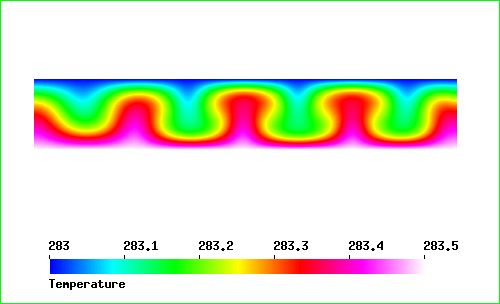
\includegraphics[width=150 mm, height=50 mm]{rb_temp}
\caption{Temperature distribution at 260 s.}\label{fg:rb_temp}
\end{figure} 

\begin{figure}[h]
\centering
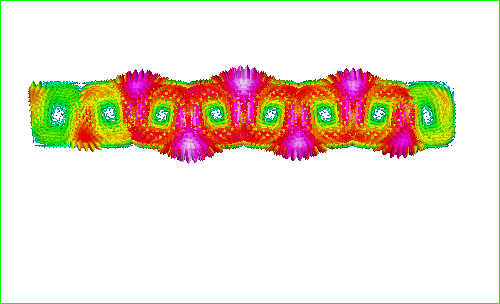
\includegraphics[width=150 mm, height=70 mm]{rb_vel}
\caption{Velocity vectors at 260 s.}\label{fg:rb_vel}
\end{figure} 
